\chapter{Remote controller}
To meet the requirement of being able to remote control the segway wirelessly and receive data from the segway wirelessly, see \autoref{requirements}, a remote controller is to be designed.\\
A wireless communication platform is needed, if data between the segway and a remote controller needs to be exchanged. As previously stated, it is desirable to remote control the segway, with respect to defining the speed and direction of the segway. Also, measurements from the segway should be possible to transmit to a remote controller where the state of the segway can be monitored. \autoref{fig:communication_intro_pic} shows the data exchanges that are desired between the segway and the remote controller.
\begin{figure}[H]
	\centering
	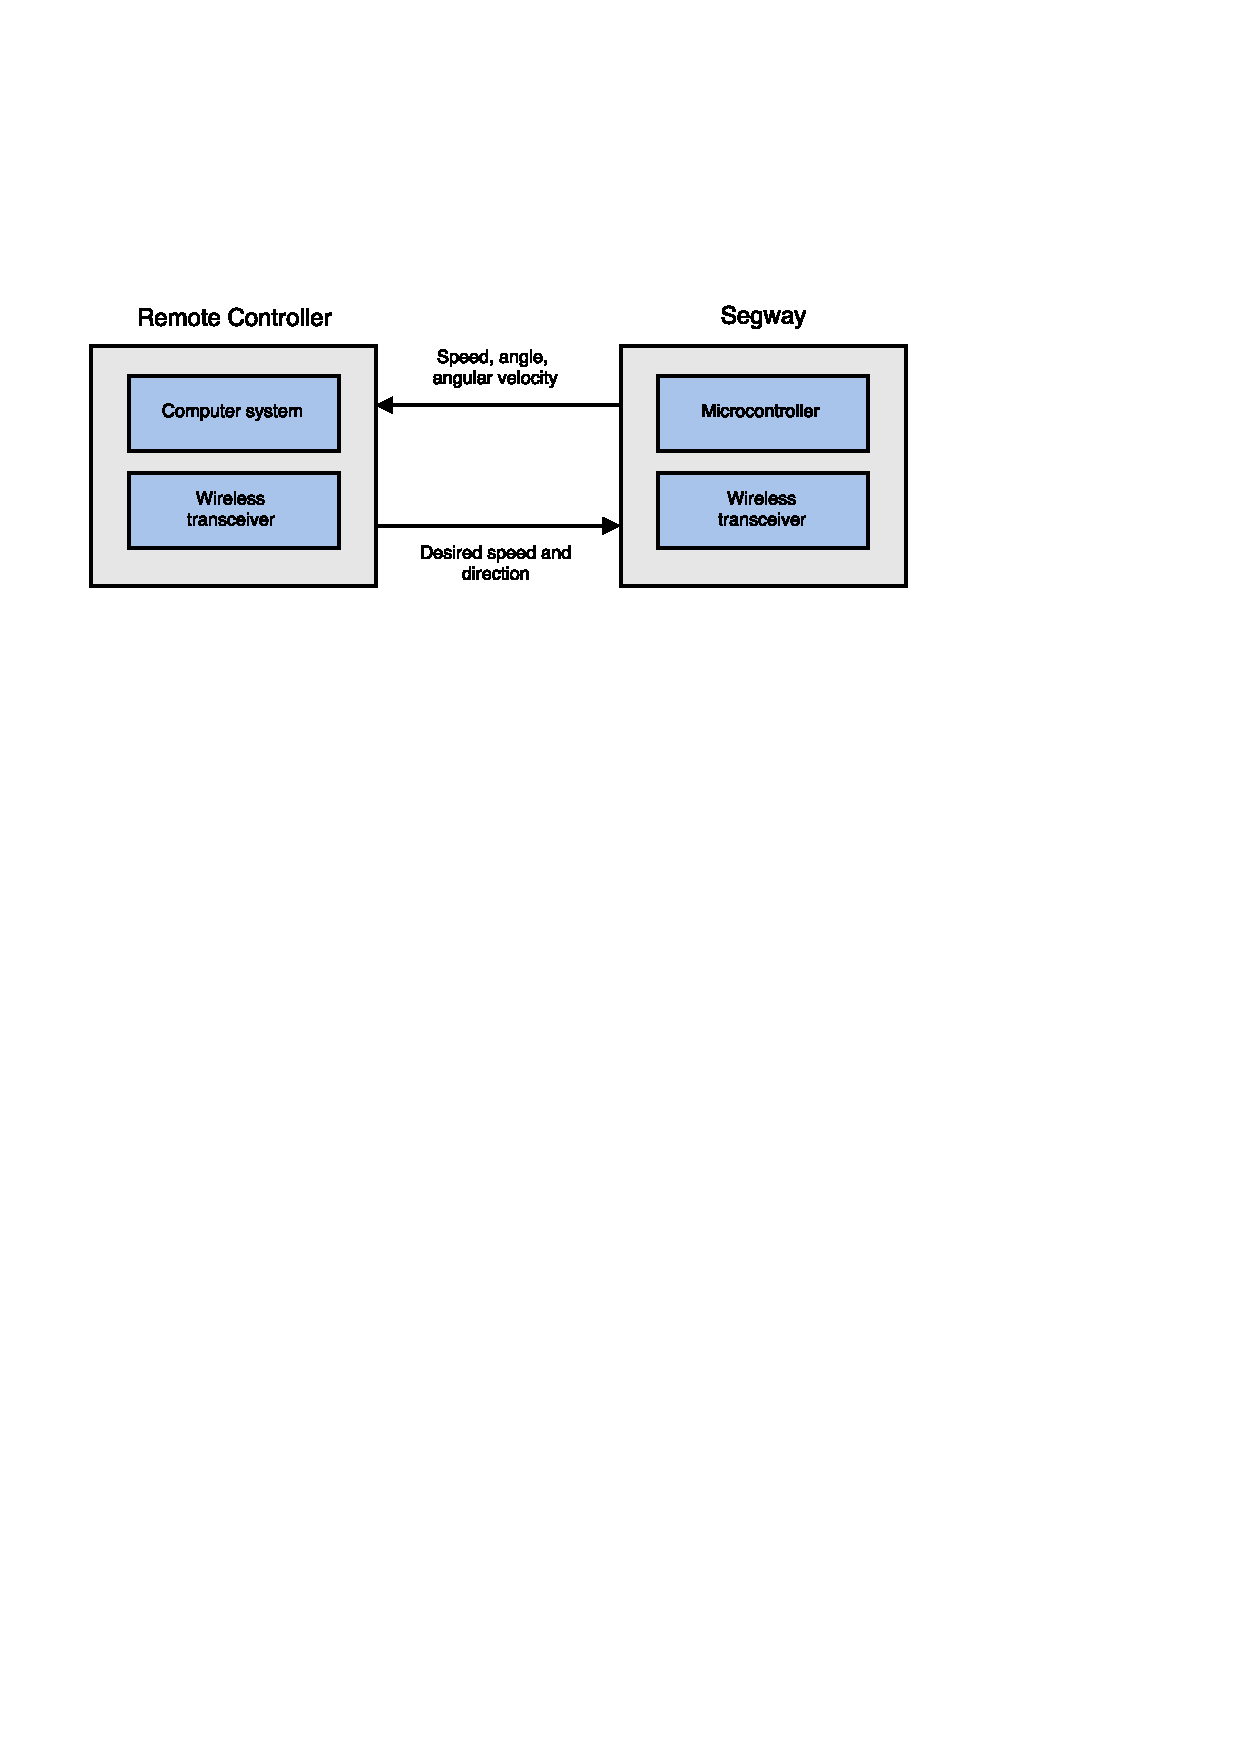
\includegraphics[width=0.7\textwidth]{figures/communication_intro_pic.pdf}
	\caption{Overview of the communication link between the remote controller and the segway.}
	\label{fig:communication_intro_pic}
\end{figure}
The remote controller should transmit the desired speed and desired direction when the user wishes to change these. To receive the current speed, inverted pendulum angle and angular velocity of the segway, the remote controller has to transmit a request to the segway, i.e. the communication will be request-based.

\section{Requirements and Specifications for the Remote Controller}

The topic of this chapter will primarily be the development of a communication protocol for data exchange between the segway and the remote controller. The requirements and specifications are thus only for the communication protocol. Based on the requirements set in \autoref{requirements}, the remote controller must be able to do the following through the communication protocol:
\begin{itemize}
\item Request the current speed, angle and angular velocity of the segway.
\item Send the desired speed and direction to the segway.
\end{itemize}

Related to this, the segway must be able to:
\begin{itemize}
\item Reply to requests for the current speed, angle and angular velocity.
\item Set the speed and direction of the segway when receiving a new reference.
\end{itemize}
In the following section, a communication protocol will be designed.

\section{Design of Communication Protocol}
To facilitate the communication between the remote controller (RC) and the segway, a communication protocol is needed. This protocol is to ensure that data is received correctly without errors, and ensures that the communication between the two devices has a certain set of rules to act within, so messages are not misunderstood.\\\\
It is decided to make the communication between the RC and segway request-based, meaning that the RC is to request some data from the segway before it is sent. This is done to reduce the computation time needed on the microcontroller on the segway for the communication, since the microcontroller  will only have to handle the communication when a request is made.
\subsection{The OSI-model}
Before designing the communication protocol, the Open Systems Interconnection (OSI) model needs to be described, as this is used for identifying the functionalities of the protocol.
The OSI model is used to describe various layers of a networking platform. The networking platform is in this case the communication between a segway and a remote controller. The OSI-model does not describe how the various communication protocols should be designed, but describes the purpose and function of each layer \citep{tanenbaum}.

\begin{table}[H]
\centering

\begin{tabular}{c}
\hline
\multicolumn{1}{|M{0.3\textwidth}|}{Application}   \\ \hline
                      %                   \\ \hline
\multicolumn{1}{|M{0.3\textwidth}|}{Presentation}  \\ \hline
                      %                   \\ \hline
\multicolumn{1}{|M{0.3\textwidth}|}{Session} \\ \hline

\multicolumn{1}{|M{0.3\textwidth}|}{Transport} \\ \hline

\multicolumn{1}{|M{0.3\textwidth}|}{Network} \\ \hline

\multicolumn{1}{|M{0.3\textwidth}|}{Data link} \\ \hline

\multicolumn{1}{|M{0.3\textwidth}|}{Physical} \\ \hline
\end{tabular}
\caption{The OSI model.}
\label{osimodel}
\end{table}

%\textbf{Physical layer} \\
%%In the physical layer, electrical
%
%\textbf{Data link layer} \\
%
%\textbf{Network layer} \\
%
%\textbf{Transport layer} \\
%
%\textbf{Session} \\
%
%\textbf{Presentation} \\
%
%\textbf{Application} \\

The OSI-model consists of seven layers, each describing the functionalities and responsibilities associated with the layer. The description of each layer will now be discussed whereupon the design choice of each layer will be clarified. 

%First, it needs to be established what the communication protocol is to handle more specifically. This is done by looking at the OSI model, see \autoref{osimodel}.

\subsubsection*{Physical Layer}
In the physical layer, the data transmission of physical signals are defined. The physical layer could concern electrical signals, frequencies or other physical sizes. The physical layer has been facilitated, since the APC220 modules used for the communication uses a wireless channel, with a frequency of about 434 MHz \citep[p. 3]{APC220}. These modules are capable of sending data using Gaussian Frequency Shift Keying (GFSK) modulation. %The modulation of GFSK is similar to FSK, where the main difference between the modulation is the Gaussian filter applied on the GFSK \citep{sou:gfsk}.
%So, all data transmitted between the modules should be split up into byte-size chunks to be transmitted one at a time.

\begin{figure}[H]
	\centering
	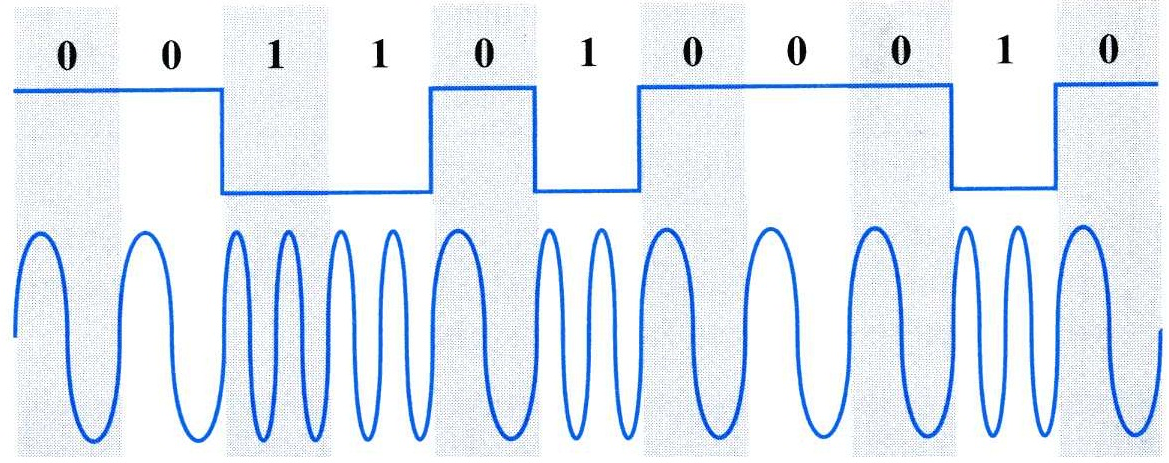
\includegraphics[width=0.7\textwidth]{figures/gfsk.png}
	\caption{FSK modulation, where the frequency is shifted dependent on the binary data sent. The difference between GFSK and FSK is the gaussian filter applied on the GFSK  \citep{sou:fsk_pic}.}
	\label{fig:fsk}
\end{figure}

GFSK means that the signal has a certain center frequency, in this case around 434 MHz, however, a slightly different frequency is used to transmit either a binary '0' or '1'. So, to send one binary data value, the center frequency is used, and to send the other binary data value, a different frequency is used. This frequency deviation can be changed in the APC220 modules, from 418 MHz to 455 MHz \citep[p. 2]{APC220}. An example of how GFSK data looks can be seen in \autoref{fig:fsk}, where the data is shown on top, and the GFSK signal in the bottom.
Gaussian Frequency Shift Keying is in this way similar to regular Frequency Shift Keying, FSK. The Gaussian in the name refers to a gaussian filter that is applied to the signal to smoothen the signal and thus reduce the rapid frequency changes seen in the FSK signal. This reduces the bandwidth of the signal, which is desired \citep{sou:gfsk}.

\subsubsection*{Data Link Layer}
The data link layer provides services to the network layer. It is responsible for the link between nodes in the network, and also handles error control. As a part of this, the data link layer is responsible for allocating the channel to avoid collisions. In this case, collision avoidance and channel allocation are not implemented. This is done because the protocol is request based. Thus, data will not be sent by the RC and segway simultaneously, since the RC will request data, wait for a reply, and then request new data. The functionality regarding error control is however implemented in the protocol, in the form of a checksum on the data transmitted.

An alternative design approach, is to make the segway transmit regularly. In contrast to the request based, the segway do not wait for a request but transmits data, for instance, every 10 ms. However this  requires that segway must use more computation time at the communication compared to the request based approach. Therefore the request based approach is chosen to be designed.

\subsubsection*{Network Layer}
The network layer is responsible for routing, i.e. sending packages from one hub in the network to another, to make it reach its destination. The network layer is also responsible for congestion control, i.e. making sure that the channel is not overloaded with data.
The features of the network layer are not implemented in the protocol. This is because only two units are connected, and thus there is no reason to have routing.

\subsubsection*{Transport Layer}
The transport layer is an end-to-end layer, meaning that units talking on the transport layer are not seeing the entire network, but only the other end. The transport layer features are somewhat implemented in the protocol, however it can be discussed if it is implemented in the transport layer or the application layer. 

In the case of the internet, there are two typical transport layer protocols used, namely TCP (Transmission Control Protocol) and UDP (User Datagram Protocol). The main difference between the two is that TCP is connection-based, i.e. a connection between hosts is set up, and then data can be sent back and forth. On the other hand, UDP is a connection-less protocol, meaning that it is individual packages that are sent back and forth.
TCP has acknowledgements and handles retransmission, to ensure that all package are received correctly, whereas UDP does not facilitate this. This means that UDP is simpler than TCP, and also has less overhead. This can be seen based on the header size, where UDP has a header size of 8 bytes, whereas TCP has a header size of at least 40 bytes \citep{tanenbaum}, meaning that for short conversations, UDP can be more efficient.

The protocol designed is somewhat similar to UDP. It is decided to make the protocol similar to UDP over TCP, to reduce the overhead, since the amount of data transmitted is not very big. Therefore, having a protocol with multiple handshakes and acknowledges is not desired, since it will require an undesirably large amount of computation from the segway.\\
Instead, a rather simple protocol with a small overhead is chosen, to minimize computation power and the amount of data sent on the channel. %This is desired, since the choice of not supporting acknowledges means that the more data is sent over the channel, the bigger the risk is of one of the bytes that is sent to have bit errors, meaning that the entire package has to been discarded. 
Another feature that is implemented in the transport layer is timeouts. The timeouts make sure that if a packet get lost under transmission, the segway or RC does not wait forever on the lost packet, but return after a set time without any response. The timeout is basically a timer that starts to count when the first byte of the packet is received. If the next packet is not received within the timeout, the function stops waiting for the next bytes and exits. Timeouts are seen as something that takes place in the transport layer, as this is the case for TCP, which will close the connection after a certain time with no data.

\subsubsection*{Session and Presentation layers}
The session and presentation layers are not used in most applications of the OSI model, since their responsibilities are not used in typical networking applications. The same is the case here, and these layers are therefore not described further. 

\subsubsection*{Application layer}
The application layer is the layer that can be used directly by the user. Here, the application layer corresponds to the actual remote controller, and the segway. This layer should see the lower layers as a black-box, meaning that to the application layer, simple functions such as \emph{RequestAngle()} and \emph{sendDesiredAngle()} should be available, without the user (in this case the programmer) thinking about how the lower layers handle these functions.


\subsection{Package design}
Now that the OSI model has been described, the actual protocol design can begin. First, the structure of the data packages sent is determined.

It is decided that a package in the communication protocol designed consists of three overall fields: A header, the data, and a footer, consisting of a checksum. This can be seen in \autoref{overallPackage}.
\begin{figure}[H]
\centering
\begin{tabular}{c}
\hline
\multicolumn{1}{|M{0.3\textwidth}|}{Header (2 bytes)}   \\ \hline
                      %                   \\ \hline
\multicolumn{1}{|M{0.3\textwidth}|}{Data (0-16 bytes)}  \\ \hline
                      %                   \\ \hline
\multicolumn{1}{|M{0.3\textwidth}|}{Checksum (2 bytes)} \\ \hline
\end{tabular}
\caption{The overall contents of a package.}
\label{overallPackage}
\end{figure}


It is optional to include data in the package, depending on whether or not this is needed - an example of this will be shown later. If no data is included in the package, the checksum-footer is not transmitted either.

The package design is inspired by the UDP header, which can be seen in \autoref{udp-header}.
\begin{table}[H]
\hspace{0.5cm}
\begin{tabular}{r|M{0.3\textwidth} M{0.3\textwidth}}
\multicolumn{1}{l}{Byte offset} |& \multicolumn{1}{l}{Bit 0}                  & \multicolumn{1}{r}{Bit 32}                      \\ \cline{2-3} 
0                                & \multicolumn{1}{M{0.3\textwidth}|}{Source port (16 bits)} & \multicolumn{1}{M{0.3\textwidth}|}{Destination Port (16 bits)} \\ \cline{2-3} 
4                                & \multicolumn{1}{M{0.3\textwidth}|}{Length (16 bits)}      & \multicolumn{1}{M{0.3\textwidth}|}{UDP Checksum (16 bits)}     \\ \cline{2-3} 
8                                & \multicolumn{2}{M{0.6\textwidth}|}{Data (if any)}                                                           \\ \cline{2-3} 
\end{tabular}
\caption{The UDP header \& data field.}
\label{udp-header}
\end{table}

From \autoref{udp-header}, it is seen that the UDP header contains 4 fields, each with a length of 16 bits: A source, a destination, the data length and a checksum. 

The contents of the header in the designed protocol can be seen in \autoref{header}. The header can be seen as consisting of two parts: The first byte containing flags, and the second byte containing the data length in bytes, i.e. one bit in the data size field represents one byte of data. \\

\begin{figure}[H]
\centering
\begin{tabular}{ccccccccc}
\cline{2-9}
Field 1 & \multicolumn{1}{|M{0.1\textwidth}|}{Reply} & \multicolumn{1}{M{0.05\textwidth}|}{$v_s$} & \multicolumn{1}{M{0.05\textwidth}|}{$\theta_P$} & \multicolumn{1}{M{0.05\textwidth}||}{$\omega_P$} & \multicolumn{1}{M{0.05\textwidth}|}{$\theta_D$} & \multicolumn{1}{M{0.05\textwidth}|}{$\phi_D$} & \multicolumn{1}{M{0.1\textwidth}|}{Reserved for future use} & \multicolumn{1}{M{0.1\textwidth}|}{Reserved for future use} \\ \cline{2-9}\cline{2-9}

Value&\multicolumn{1}{|M{0.1\textwidth}|}{0} & \multicolumn{1}{M{0.05\textwidth}|}{0} & \multicolumn{1}{M{0.05\textwidth}|}{0} & \multicolumn{1}{M{0.05\textwidth}||}{0} & \multicolumn{1}{M{0.05\textwidth}|}{0} & \multicolumn{1}{M{0.05\textwidth}|}{0} & \multicolumn{1}{M{0.1\textwidth}|}{1} & \multicolumn{1}{M{0.1\textwidth}|}{1} \\ \cline{2-9}
\\ \cline{2-9}
Field 2&\multicolumn{8}{|c|}{Data size}                                                                                                                                                                                                                                                                 \\ \cline{2-9}
\end{tabular}
\caption{The header contents of a single package. Field 1 is the first header byte, while field 2 is the second header byte.}
\label{header}
\end{figure}

The flags are somewhat similar to the destination and source fields in the UDP header, as they describe what the receiver, i.e. the segway, should do with the data, e.g. reply with the measured angle or set a new reference angle. The UDP length is also included in the protocol, by means of the second header byte. The UDP checksum is also included in the package, but is made as a footer instead as a part of the header. The checksum is therefore only added to the data, and not the header, to reduce the overhead, since the checksum is only sent if data is sent. This is a fair choice to make, because the risk of bit errors in the header is smaller than that on the data, since the header is only two bytes long.

The first bit of the header is a reply field. When the bit is set to '0' the RC transmits a request to the segway. The segway then performs the requested actions and afterwards responds by transmitting a packet to RC, where the first bit is set to '1'. %The bit is set to '0' when the RC is requesting data from the segway or sending it new reference values, and set to a '1' when the segway is sending a reply. 
The next three bits are flags, showing which data is either requested or not. The options are the segway speed, $v_s$, the segway tilting angle, $\theta_p$ and the angular velocity of the segway, $\omega_p$. Each of these fields can be set, to indicate the data requested/transmitted. If for example the segway speed is requested, $v_s$, the second bit in the first header is set to '1'.
When the segway is replying with the data values, the data size field is updated accordingly.
The segway tilting angle, $\theta_p$, and the angular velocity of the segway, $\omega_p$, both have a size of 4 bytes, since the value transmitted is a float. The segway speed takes up 8 bytes, as it is two floats that are transmitted, namely the speed of both left and right motor.
The values sent could be converted into a 16-bit integer, as all data in the microcontroller on the segway is sampled using at maximum 16 bit, to reduce the amount of data sent. However, for simplicity, the numbers are kept floats as this is the data type that the values are used as in the microcontroller.\\
The next two header bits are the desired speed $\theta_D$, and the desired turning angle of the segway, $\phi_D$. These fields are set by the RC, if the user wants to change these reference values for the segway, to either make the segway go forward, backwards or turn it. Each of these values have a size of 4 bytes, a float, and when transmitted, the data size field must be updated accordingly.
Finally, the last two bits of the first header byte are not used, and are set to a '1'.

Looking at \autoref{overallPackage}, after the header is transmitted, which describes which data is sent and the length of that data, the actual data is transmitted. The data will have a maximum size of 16 byte, which occurs if the segway is to send both $v_s$, $\theta_P$ and $\omega_p$. 

Finally, a 16 bit cyclic redundancy check (CRC-16) checksum is added in the end of the frame, to verify that the data sent has been received correctly. To determine if the package do not contain errors, the checksum is compared to the received data. The details of the method behind the CRC-16 code will not be explained here, but the process of generating the checksum can be seen as a polynomial division, where the remainder is the checksum. The CRC16-code generator and CRC-16 checker can be found here \citep{jdn}. 
If the CRC-16 code does not match up with the data received, the package is discarded, and it is up to the user to either ask for the data again or just ignore the lost data. The datasheet for the APC220 states, the module has a high efficiently error correction implemented \citep[p. 8]{APC220}. However the checksum has been chosen to be implemented for better error detection.

An example of a the headers sent during a transmission consisting of a request and reply can be seen in \autoref{fig:transmission}.

\begin{figure}[H]
\hspace{0cm}
\centering
\scalebox{0.80}{
\begin{tabular}{ccccccccc}
\multicolumn{9}{c}{Remote controller requesting angular position and angular velocity.}                                                                                                                                                                                                                                                          \\
\multicolumn{9}{c}{}                                                                                                                                                                                                                                                          \\
\cline{2-9}
Field 1 & \multicolumn{1}{|M{0.1\textwidth}|}{Reply} & \multicolumn{1}{M{0.05\textwidth}|}{$v_s$} & \multicolumn{1}{M{0.05\textwidth}|}{$\theta_P$} & \multicolumn{1}{M{0.05\textwidth}||}{$\omega_P$} & \multicolumn{1}{M{0.05\textwidth}|}{$\theta_D$} & \multicolumn{1}{M{0.05\textwidth}|}{$\phi_D$} & \multicolumn{1}{M{0.1\textwidth}|}{Reserved} & \multicolumn{1}{M{0.1\textwidth}|}{Reserved} \\ \cline{2-9}\cline{2-9}

Value&\multicolumn{1}{|M{0.1\textwidth}|}{0} & \multicolumn{1}{M{0.05\textwidth}|}{0} & \multicolumn{1}{M{0.05\textwidth}|}{1} & \multicolumn{1}{M{0.05\textwidth}||}{1} & \multicolumn{1}{M{0.05\textwidth}|}{0} & \multicolumn{1}{M{0.05\textwidth}|}{0} & \multicolumn{1}{M{0.1\textwidth}|}{1} & \multicolumn{1}{M{0.1\textwidth}|}{1} \\ \cline{2-9}
\\ \cline{2-9}
Field 2&\multicolumn{8}{|c|}{0}                                                                                                                                                                                                                                                                 \\ \cline{2-9}
\end{tabular}
}

\scalebox{0.80}{\centering
\begin{tabular}{ccccccccc}
\multicolumn{9}{c}{}                                                                                                                                                                                                                                                          \\
\multicolumn{9}{c}{}                                                                                                                                                                                                                                                          \\
\multicolumn{9}{c}{Segway replying with angular position and angular velocity.}                                                                                                                                                                                                                                                          \\
\multicolumn{9}{c}{}                                                                                                                                                                                                                                                          \\
\cline{2-9}
Field 1 & \multicolumn{1}{|M{0.1\textwidth}|}{Reply} & \multicolumn{1}{M{0.05\textwidth}|}{$v_s$} & \multicolumn{1}{M{0.05\textwidth}|}{$\theta_P$} & \multicolumn{1}{M{0.05\textwidth}||}{$\omega_P$} & \multicolumn{1}{M{0.05\textwidth}|}{$\theta_D$} & \multicolumn{1}{M{0.05\textwidth}|}{$\phi_D$} & \multicolumn{1}{M{0.1\textwidth}|}{Reserved} & \multicolumn{1}{M{0.1\textwidth}|}{Reserved} \\ \cline{2-9}\cline{2-9}

Value&\multicolumn{1}{|M{0.1\textwidth}|}{1} & \multicolumn{1}{M{0.05\textwidth}|}{0} & \multicolumn{1}{M{0.05\textwidth}|}{1} & \multicolumn{1}{M{0.05\textwidth}||}{1} & \multicolumn{1}{M{0.05\textwidth}|}{0} & \multicolumn{1}{M{0.05\textwidth}|}{0} & \multicolumn{1}{M{0.1\textwidth}|}{1} & \multicolumn{1}{M{0.1\textwidth}|}{1} \\ \cline{2-9}
\\ \cline{2-9}
Field 2&\multicolumn{8}{|c|}{8}                                                                                                                                                                                                                                                                 \\ \cline{2-9}
\end{tabular}
}
\caption{The headers of a data transmission consisting of a request and a reply.}
\label{fig:transmission}
\end{figure}

In the example above, the user wants to receive data regarding the segway's angle and angular velocity. Bit 3 and 4 in the first header is therefore set to '1' to indicate so. The second header byte is set to 0 since no data from the user needs to be transmitted to the segway. When the segway receives the request, it responds by transmitting two header bytes where the first header byte indicates it is a reply and the second header byte that the incoming data is 8 bytes long, respectively 4 bytes for the angle and 4 bytes for the angular velocity. After transmitting the header bytes, the 8 data bytes are transmitted, followed by the 2 byte footer, which are now shown. 
It is possible that a byte gets lost under transmission. To avoid the segway waiting forever on a lost byte, a timeout is implemented which exits the process, if a certain time has expired without any reply has been received. I.e. if the segway waits on the second header byte but the byte is lost, the timeout ensures that the read function returns a 1 meaning the package is lost, whereas a 0 is returned if the package was received successfully. This way, the functions calling the read function can handle the received data or return an error if no data is received.

Examples of two transmissions can be seen in \autoref{reqAngleFig} and \ref{reqAngularFig}. In \autoref{reqAngleFig}, it is seen how the remote controller requests for $\theta_p$ and is sent over the channel. When the segway receives the request, it replies with transmitting $\theta_p$, which is the request angle to the user.

\begin{figure}[H]
\centering
\input{figures/reqAngle.ralf}
\caption{The communication for when the RC requests the current segway angle.}
\label{reqAngleFig}
\end{figure}

In \autoref{reqAngularFig} the RC requests $\omega_p$, but the reply is lost. This causes the RC to timeout, as it is waiting for a reply within a certain time. Since the reply was not received, the function timeouts, and returns an error message, 0xFFFF, to show that no reply was received. The user can then choose to either ignore this, or try to request the data again.

\begin{figure}[H]
\centering
\input{figures/reqAngularVelocity.ralf}
\caption{The RC requests the segway angular velocity, but the reply is lost.}
\label{reqAngularFig}
\end{figure}

%\begin{figure}[H]
%\centering
%\input{figures/setDesiredTurn.ralf}
%\caption{The communication for when the RC changes the desired turning angle on the segway.}
%\label{setTurnFig}
%\end{figure}
\newpage
\section{Implementation of wireless communication}
The implementation of the designed communication protocol and remote controller is explained in this section. The structure of the following section is to first explain the low level implementation and then move to higher level implementation.% For instance, before explaining the implementation of the communication protocol, basic communication between the segway and RC needs to be established and implemented, i.e. it is possible to transmit and receive a byte between the segway and RC.
 
The APC220 modules, i.e. the radio modules used for the communication, use UART to serial communication with the segway and RC. The default baud rate for the UART module on the APC220's is 19200 baud. Therefore, the baud rate on the UART modules on the segway and RC are set to 19200 as well. It should be mentioned that the serial communication between the APC220 and the segway is handled by an external UART module on the XMEGA128 chip, and not by the microcontroller itself. 

The first step of implementation is to establish communications between the APC220 transceiver module on the RC with the segway. Two basic driver functions for the APC220 are both implemented on the segway and RC. These functions ensure receiving and transmission of data, and are named \textit{APC220\_SEND()} and \textit{APC220\_READ()}. %For the segway, the functions are implemented in the c-file segway\_func.c.
The implemented code can be seen in \autoref{lst:APC220driversegway}.

\lstset{language=C, caption={APC220 driver for segway.}, label=lst:APC220driversegway}
\begin{lstlisting}
void APC220_SEND(uint8_t APC220_SEND_DATA){
	uartWriteChar(APC220_SEND_DATA);	// Transmit a byte through UART TX
}

uint8_t APC220_READ(uint8_t *APC220_READ_DATA){
	int timer = 0;
	while (uartAvailable() == 0 && timer++ < TIMEOUT); // Timeout counter
	if(timer < TIMEOUT){
		*APC220_READ_DATA = uartRead();	// Read data from UART RX
		return 0;	
	}
	return 1;
}
\end{lstlisting}

When the UART RX buffer on the segway has received data from the APC220 module, an interrupt service rutine (ISR) is triggered to set a flag high, stating there is data in the UART RX buffer. The main code will check if this flag is set, and if that is the case, it will handle the information received. 
A similar APC220 driver is implemented on the RC. With the implemented APC220 UART drivers, it is now possible to transmit and receive bytes through the APC220 modules. These driver functions will be used to transmit and receive the header bytes and data bytes. With the send and read driver functions for the APC220 working, it is now possible to proceed with implementing the communication protocol. 

The implemented communication protocol can be seen in \autoref{lst:func_protocol}. The structure of the protocol is split into high level and low level functions.\newpage
\lstset{language=C, caption={Functions used for the communication protocol.}, label=lst:func_protocol}
\begin{lstlisting}
//		HIGH LEVEL FUNCTIONS
float requestSpeed();
float requestAngle();
float requestAngularVelocity();
void sendDesiredAngle(float desiredAngle);
void sendDesiredTurn(float desiredTurn);

//		LOW LEVEL FUNCTIONS
int ReceivePackage(void);
void extractDatafromSignal(uint8_t *header, uint8_t *inData);
void handleTransmitRequest();
void sendSpeed(uint8_t dataIndex);
void sendAngle(uint8_t dataIndex);
void sendAngularVelocity(uint8_t dataIndex);
int transmitPackage(); 
int dataReceivedHandler();
void handleTransmitRequestSegway();
\end{lstlisting}
The high level functions are used by the user, and can be called from the main code. Through the high level functions it is, for instance, possible to request the current speed of the seqway by calling the \textit{requestAngle()} function. The function then returns the speed of the segway when the RC has received a response from the segway. The low level functions are handled by the high level functions, and should not be called by the user. The contents of the low level functions are primary extracting information from the received packages, and making sure that transmissions comply with the protocol. The high level functions perform call to the lower level drivers, i.e. by transmitting a request and returning the value that was replied from the segway.

The last part in the implementation is how to handle the high level function from the main file for the RC and segway. It is straight forward to handle the high level function from the RC, since the only thing required is to simply call one of the high level functions from \autoref{lst:func_protocol}. On the segway, a flag is used to indicate if there is data in the UART RX buffer. If the UART RX buffer is not empty the function \textit{dataReceivedHandler()} is called to read the package. Afterwards, the function \textit{handleTransmitRequestSegway()} is called to perform the desired action from the RC, e.g. to transmit the tilting angle or set a new speed reference. \autoref{lst:receive_data} shows the implemented code main code for the communication on the segway side.

\lstset{language=C, caption={Read and handle the data from the UART buffer on the segway.}, label=lst:receive_data}
\begin{lstlisting}
if(RECEIVE_FLAG()){
	if(dataReceivedHandler() == 0){
		handleTransmitRequestSegway();
	}
	SET_RECEIVE_FLAG(0);
}
\end{lstlisting}

The communication protocol is now designed and implemented and can now be used for communicating between the segway and RC.












